\chapter{Последовательности и прогрессии}\label{chap:c12-progressions}\markright{Глава 16}
\begin{definition}
\term{Числовая последовательность} (real sequence) — отображение \(a:\mathbb N\to\mathbb R\), где \(\mathbb N=\{1,2,3,\ldots\}\). Числу \(n\) соответствует \term{член последовательности} (term) \(a_n\); \(n\) — его номер. Последовательность записывают как \((a_n)_{n\geq1}\).
\end{definition}
\begin{definition}
\term{Формула общего члена} (explicit formula) непосредственно выражает \(a_n\) через \(n\). \term{Рекуррентная, или индуктивная, запись} (recursive definition) задаёт начальное значение и правило получения следующих членов из предыдущих. Например, \(a_1=2\), \(a_{n+1}=a_n+3\) при \(n\geq1\).
\end{definition}
\begin{definition}
\term{Арифметическая прогрессия} (arithmetic progression) — последовательность, для которой \(a_{n+1}=a_n+d\) при всех \(n\geq1\). Постоянное число \(d\) называют \term{разностью прогрессии} (common difference).
\end{definition}
\begin{theorem}[Общий член арифметической прогрессии]\label{thm:legacy-c12-1}
Для арифметической прогрессии
\[
a_n=a_1+(n-1)d,\qquad n\geq1.
\]
\end{theorem}
\begin{proof}
При \(n=1\) равенство верно. Если \(a_k=a_1+(k-1)d\), то \(a_{k+1}=a_k+d=a_1+kd\). По математической индукции формула верна для всех \(n\geq1\).
\end{proof}
\begin{definition}
\term{Частичная сумма} (partial sum) последовательности — сумма первых \(N\) членов: \(S_N=a_1+\cdots+a_N\).
\end{definition}
\begin{theorem}[Сумма арифметической прогрессии]\label{thm:legacy-c12-2}
\[
S_N=\frac{N(a_1+a_N)}{2}=\frac N2\bigl(2a_1+(N-1)d\bigr).
\]
\end{theorem}
\par\addvspace{5pt}\begin{lrbox}{\CatFlowBox}\begin{minipage}[t]{\linewidth}
\setlength{\parskip}{5pt}\setlength{\columnsep}{4.5mm}\setlength{\intextsep}{0pt}
\begin{wrapfigure}[12]{l}{54mm}
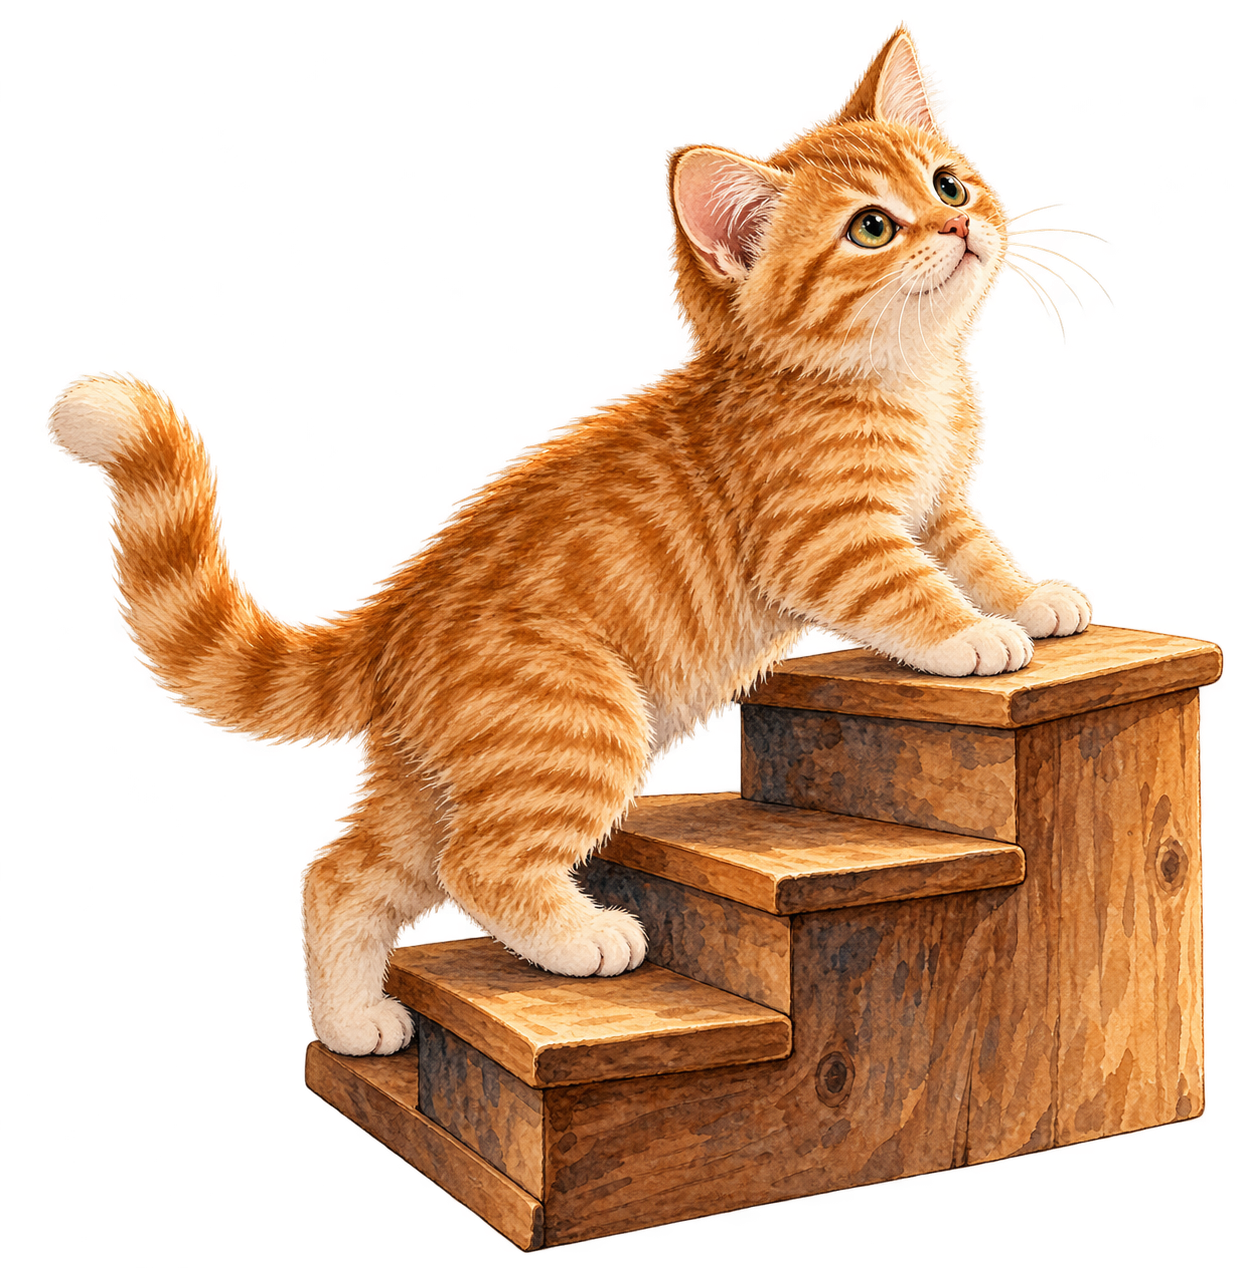
\includegraphics[width=54mm,height=58mm,keepaspectratio]{images/unique/art-13.png}
\label{catflow:13}
\end{wrapfigure}
\textit{Доказательство.} Запишем одну и ту же сумму в прямом и обратном порядке. При сложении получим \(2S_N=(a_1+a_N)+(a_2+a_{N-1})+\cdots+(a_N+a_1)\). В каждой из \(N\) скобок сумма равна \(2a_1+(N-1)d=a_1+a_N\). Деление на \(2\) даёт первую формулу, а подстановка общего члена — вторую. Рассуждение не зависит от чётности \(N\).\hfill\(\blacksquare\)
\par\WFclear\end{minipage}\end{lrbox}%
\ifdim\dimexpr\ht\CatFlowBox+\dp\CatFlowBox\relax<64mm\dp\CatFlowBox=\dimexpr64mm-\ht\CatFlowBox\relax\fi%
\noindent\usebox{\CatFlowBox}\par\addvspace{5pt}

\begin{definition}
\term{Геометрическая прогрессия} (geometric progression) в этом сборнике — последовательность, для которой \(a_{n+1}=q a_n\) при всех \(n\geq1\). Постоянное число \(q\) называют \term{знаменателем прогрессии} (common ratio). Такое определение включает \(q=0\): тогда последовательность имеет вид \(a_1,0,0,\ldots\).
\end{definition}
\begin{theorem}[Общий член геометрической прогрессии]\label{thm:legacy-c12-3}
При \(q\neq0\)
\[
a_n=a_1q^{n-1},\qquad n\geq1.
\]
При \(q=0\) отдельно имеем \(a_n=0\) для \(n\geq2\); значение \(a_1\) задано начальным условием.
\end{theorem}
\begin{proof}
При \(q\neq0\) база \(n=1\) даёт \(a_1q^0=a_1\). Из формулы для \(k\) следует \(a_{k+1}=q a_k=q a_1q^{k-1}=a_1q^k\). При \(q=0\) сначала \(a_2=0\), затем каждый следующий член равен \(0\cdot0=0\). Такое отдельное рассмотрение позволяет не использовать неопределённую запись \(0^0\).
\end{proof}
\begin{theorem}[Сумма геометрической прогрессии]\label{thm:legacy-c12-4}
При \(q\neq1\)
\[
S_N=\frac{a_1(1-q^N)}{1-q}.
\]
При \(q=1\) имеем \(S_N=Na_1\). Формула для \(q\neq1\) верна также при \(q=0\).
\end{theorem}
\begin{proof}
Из рекуррентного правила
\(qS_N=a_2+a_3+\cdots+a_{N+1}\). Вычитая это равенство из \(S_N=a_1+a_2+\cdots+a_N\), получаем \((1-q)S_N=a_1-a_{N+1}=a_1(1-q^N)\). При \(q\neq1\) делим на \(1-q\). При \(q=1\) все члены равны \(a_1\), поэтому сумма равна \(Na_1\).
\end{proof}

\section{Примеры: явное и рекуррентное задание}
\begin{example}Пусть \(a_1=3\), \(a_{n+1}=a_n+4\). Последовательно получаем \(3,7,11,15,\ldots\). Каждый переход прибавляет четвёрку, поэтому \(a_n=3+4(n-1)=4n-1\); это проверяется индукцией. Десятый член \(39\), сумма первых десяти \(S_{10}=\frac{10(3+39)}2=210\). Рекуррентное правило удобно для следующего шага, а явное --- для члена с большим номером.\end{example}
\begin{example}Пусть \(b_1=2\), \(b_{n+1}=3b_n\). Первые члены \(2,6,18,54\), а \(b_n=2\cdot3^{n-1}\). Сумма первых четырёх \(S_4=\frac{2(3^4-1)}{3-1}=80\). Проверка сложением: \(2+6+18+54=80\). В формуле суммы требуется отдельный случай \(q=1\): тогда \(S_n=nb_1\), поскольку делить на \(q-1=0\) нельзя.\end{example}
\Needspace{7\baselineskip}\section*{Задачи}
\begingroup\setlength{\parskip}{2pt}
\noindent\begin{minipage}[t]{\linewidth}\textbf{16.1.} Последовательность задана формулой \(a_n=3n-2\), \(n\geq1\). Выпишите первые пять членов и найдите \(a_{10}\).\par\end{minipage}\par
\noindent\begin{minipage}[t]{\linewidth}\textbf{16.2.} Для \(a_n=\dfrac{(-1)^n}{n}\) выпишите первые четыре члена. Укажите знак \(a_{25}\) и знак \(a_{26}\).\par\end{minipage}\par
\noindent\begin{minipage}[t]{\linewidth}\textbf{16.3.} Дано \(a_1=2\), \(a_{n+1}=2a_n-1\). Выпишите первые пять членов последовательности.\par\end{minipage}\par
\noindent\begin{minipage}[t]{\linewidth}\textbf{16.4.} Последовательность \(3,7,11,15,\ldots\) — арифметическая прогрессия. Найдите её разность и формулу общего члена.\par\end{minipage}\par
\noindent\begin{minipage}[t]{\linewidth}\textbf{16.5.} В арифметической прогрессии \(a_1=7\), \(d=-3\). Найдите \(a_8\).\par\end{minipage}\par
\noindent\begin{minipage}[t]{\linewidth}\textbf{16.6.} В арифметической прогрессии \(a_3=11\), \(a_9=35\). Найдите \(d\) и \(a_1\).\par\end{minipage}\par
\noindent\begin{minipage}[t]{\linewidth}\textbf{16.7.} Найдите сумму первых двадцати членов арифметической прогрессии с \(a_1=5\) и \(d=2\).\par\end{minipage}\par
\noindent\begin{minipage}[t]{\linewidth}\textbf{16.8.} Последовательность \(3,-6,12,-24,\ldots\) — геометрическая прогрессия. Найдите \(q\), формулу \(a_n\) и \(a_6\).\par\end{minipage}\par
\noindent\begin{minipage}[t]{\linewidth}\textbf{16.9.} В геометрической прогрессии \(a_1=81\), \(q=\dfrac13\). Найдите \(a_5\).\par\end{minipage}\par
\noindent\begin{minipage}[t]{\linewidth}\textbf{16.10.} В действительной геометрической прогрессии \(a_2=6\), \(a_5=48\). Найдите \(q\) и \(a_1\).\par\end{minipage}\par
\noindent\begin{minipage}[t]{\linewidth}\textbf{16.11.} Вычислите сумму \(1+2+4+\cdots+128\). Сначала определите число слагаемых.\par\end{minipage}\par
\par\addvspace{2pt}\begin{lrbox}{\CatFlowBox}\begin{minipage}[t]{\linewidth}
\setlength{\parskip}{2pt}\setlength{\columnsep}{4.5mm}\setlength{\intextsep}{0pt}
\begin{wrapfigure}[9]{r}{54mm}

\includegraphics[width=54mm,height=58mm,keepaspectratio]{images/unique/art-208.png}
\label{catflow:208}
\end{wrapfigure}
\textbf{16.12.} В первую неделю в копилку положили \(100\) рублей, а в каждую следующую — на \(50\) рублей больше, чем в предыдущую. Сколько рублей положили за \(12\) недель?\par

\textbf{16.13.} В первом ряду зала \(12\) мест, а в каждом следующем на \(2\) места больше. Всего \(20\) рядов. Найдите число мест в последнем ряду и во всём зале.\par

\textbf{16.14.} В игре за первый день дают \(2\) монеты, а каждый следующий день награду удваивают. Найдите награду за седьмой день и общее число монет за первые семь дней.\par

\textbf{16.15.} Докажите с помощью формулы суммы арифметической прогрессии, что \(1+3+5+\cdots+(2N-1)=N^2\) для любого натурального \(N\).\par

\textbf{16.16.}\starmark{} Дано \(a_1=3\), \(a_{n+1}=2a_n+1\). Найдите формулу общего члена и сумму первых десяти членов.\par

\textbf{16.17.}\starmark{} В арифметической прогрессии \(d>0\), \(a_2+a_5=34\), \(a_3a_4=280\). Найдите \(a_1\), \(d\) и \(S_{10}\).\par
\par\WFclear\end{minipage}\end{lrbox}%
\ifdim\dimexpr\ht\CatFlowBox+\dp\CatFlowBox\relax<58mm\dp\CatFlowBox=\dimexpr58mm-\ht\CatFlowBox\relax\fi%
\noindent\usebox{\CatFlowBox}\par\addvspace{2pt}

\par\Needspace{12\baselineskip}\section*{Олимпиадные задачи}
\par\addvspace{2pt}\begin{lrbox}{\CatFlowBox}\begin{minipage}[t]{\linewidth}
\setlength{\parskip}{2pt}\setlength{\columnsep}{4.5mm}\setlength{\intextsep}{0pt}
\begin{wrapfigure}[11]{l}{54mm}
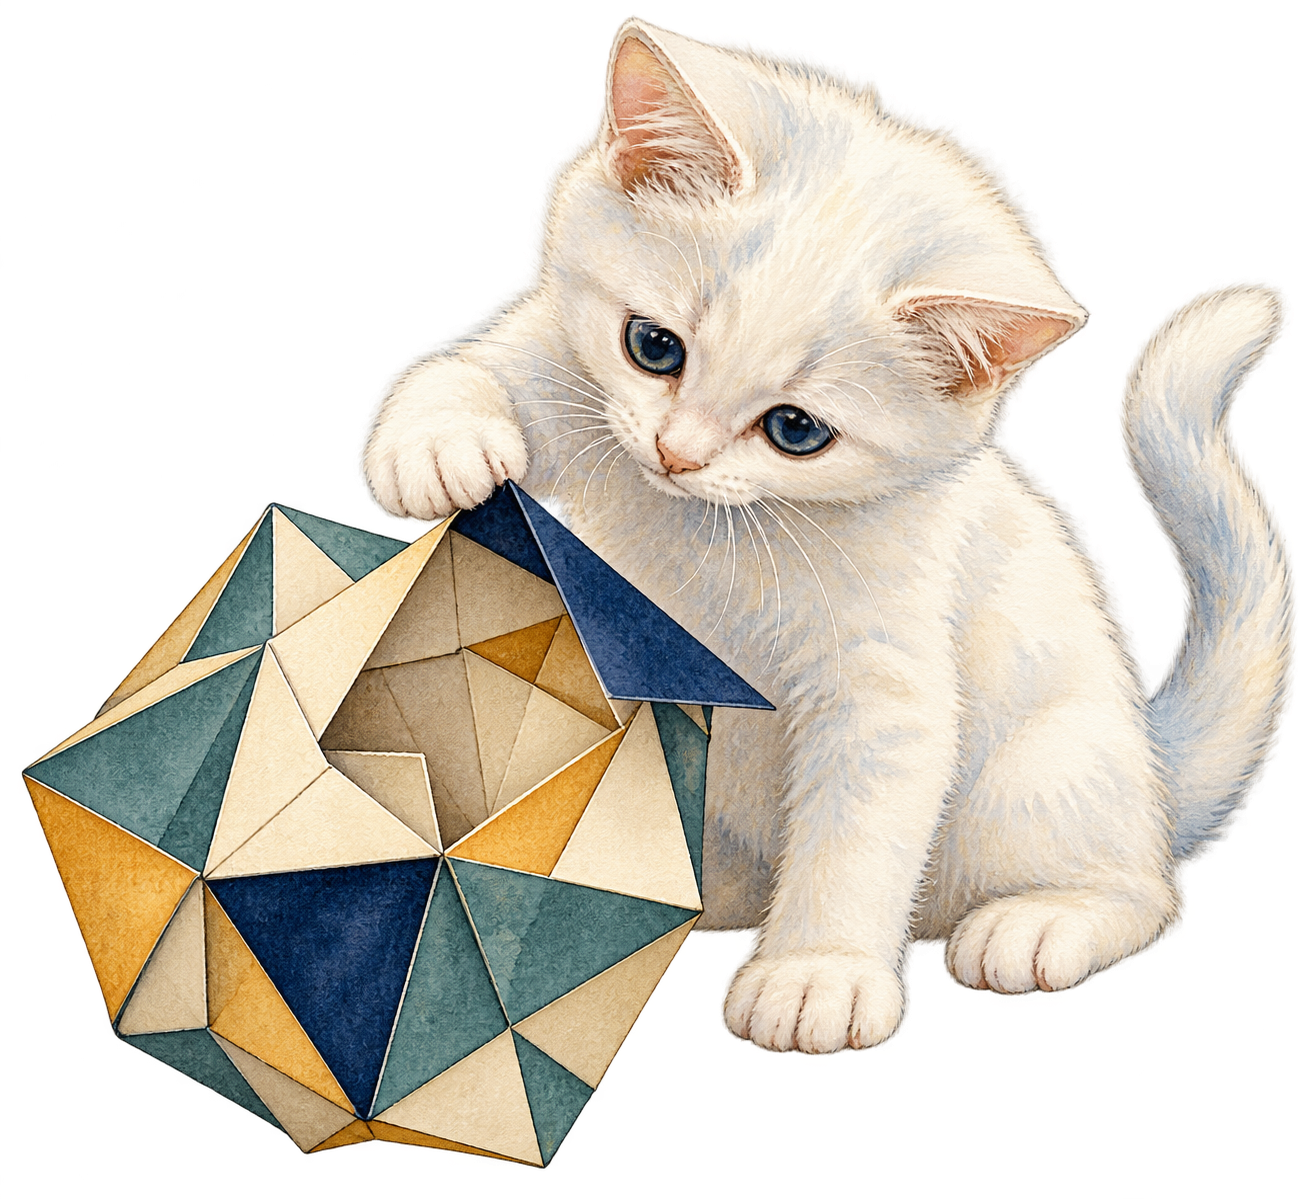
\includegraphics[width=54mm,height=58mm,keepaspectratio]{images/unique/art-303.png}
\label{catflow:303}
\end{wrapfigure}
\textbf{16.18.}\starmark{} {\small\itshape\href{https://mmo.mccme.ru/books/mmo-35-57.pdf}{ММО, 1935, I тур, вариант 3, № 1}; редакция условия.}\par Найди две действительные прогрессии, арифметическую и геометрическую, по четыре члена в каждой, если суммы соответствующих членов равны \(27,27,39,87\).\par

\textbf{16.19.}\starmark{} {\small\itshape\href{https://www.apmo-official.org/static/problems/apmo1992_prb.pdf}{APMO, 1992, № 1}; перевод.}\par Из сторон треугольника \(a,b,c\) получают новую тройку \(s-a,s-b,s-c\), где \(s=\dfrac{a+b+c}2\), и повторяют преобразование, пока новая тройка задаёт невырожденный треугольник. Для каких исходных треугольников процесс бесконечен? Напомним: положительные \(a,b,c\) задают такой треугольник тогда и только тогда, когда каждая сторона меньше суммы двух других.\par
\par\WFclear\end{minipage}\end{lrbox}%
\ifdim\dimexpr\ht\CatFlowBox+\dp\CatFlowBox\relax<58mm\dp\CatFlowBox=\dimexpr58mm-\ht\CatFlowBox\relax\fi%
\noindent\usebox{\CatFlowBox}\par\addvspace{2pt}

\endgroup
